\documentclass[12pt,a4paper]{report}

\usepackage[a4paper,margin=1in]{geometry}
\usepackage[T1]{fontenc}
\usepackage[utf8]{inputenc}
\usepackage{lmodern}
\usepackage{microtype}
\usepackage{graphicx}
\usepackage{xcolor}
\usepackage{booktabs}
\usepackage{longtable}
\usepackage{array}
\usepackage{enumitem}
\usepackage{float}
\usepackage{hyperref}
\usepackage{listings}
\usepackage{tikz}
\usepackage{fancyhdr}
\usepackage{setspace}
\usepackage{titlesec}

\usetikzlibrary{arrows.meta, positioning, shapes.geometric, fit, backgrounds}

\definecolor{primary}{HTML}{1A365D}
\definecolor{secondary}{HTML}{2B6CB0}
\definecolor{codegray}{HTML}{F3F4F6}
\definecolor{codegreen}{HTML}{166534}
\definecolor{codeblue}{HTML}{1D4ED8}

\hypersetup{
    colorlinks=true,
    linkcolor=primary,
    urlcolor=secondary,
    citecolor=secondary,
    pdftitle={AI Ergonomics and Digital-Wellness Monitoring System},
    pdfauthor={Major Project Team}
}

\lstset{
    basicstyle=\ttfamily\small,
    backgroundcolor=\color{codegray},
    frame=single,
    rulecolor=\color{black!20},
    breaklines=true,
    columns=fullflexible,
    keywordstyle=\color{codeblue},
    commentstyle=\color{codegreen},
    showstringspaces=false
}

\pagestyle{fancy}
\fancyhf{}
\lhead{\small AI Ergonomics Monitoring System}
\rhead{\small Project Report}
\cfoot{\thepage}
\setlength{\headheight}{15pt}
\onehalfspacing

\titleformat{\chapter}[display]
  {\normalfont\bfseries\color{primary}}
  {\chaptertitlename\ \thechapter}{12pt}{\Huge}
\titleformat{\section}{\normalfont\Large\bfseries\color{secondary}}{\thesection}{1em}{}
\titleformat{\subsection}{\normalfont\large\bfseries\color{primary}}{\thesubsection}{1em}{}

\newcommand{\systemname}{AI Ergonomics and Digital-Wellness Monitoring System}
\newcommand{\code}[1]{\texttt{#1}}

\begin{document}

\begin{titlepage}
\centering
\vspace*{1cm}
{\Large\bfseries Major Project\par}
\vspace{1.5cm}
{\Huge\bfseries \systemname\par}
\vspace{0.7cm}
{\Large Project Report\par}
\vspace{1.5cm}
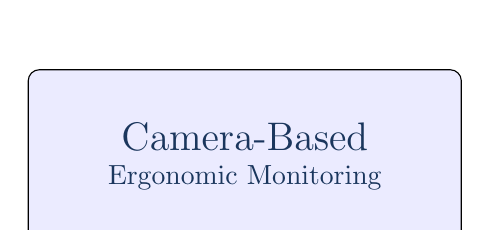
\begin{tikzpicture}
\node[draw, rounded corners, fill=blue!8, minimum width=55mm, minimum height=22mm,
      align=center, text=primary] {\Large Camera-Based\\Ergonomic Monitoring};
\end{tikzpicture}\par
\vspace{1.2cm}
{\large A real-time computer-vision platform for posture, screen-distance, and digital-wellness monitoring\par}
\vfill
\begin{tabular}{rl}
\textbf{Document type:} & Technical project report\\
\textbf{Primary implementation:} & Python, Flask, OpenCV, MediaPipe\\
\textbf{Client:} & React 19 web dashboard\\
\textbf{Persistence:} & MongoDB and GridFS\\
\textbf{Report source:} & LaTeX\\
\textbf{Version:} & 1.0\\
\end{tabular}
\vfill
{\large \today\par}
\end{titlepage}

\chapter*{Abstract}
\addcontentsline{toc}{chapter}{Abstract}
The \systemname{} is a camera-based software system that monitors posture and
digital-wellness indicators while a person works at a computer. The system
combines face and pose landmarks, calibrated screen-distance estimation,
temporal safety policies, live video delivery, session analytics, and generated
ergonomic reports. It is designed to provide actionable feedback without
requiring wearable hardware.

The implementation uses a MediaPipe-based vision pipeline for face and pose
features, an OpenCV capture layer, a temporal safety engine, and a Flask API
with WebRTC and MJPEG delivery options. A React dashboard provides live
metrics, notifications, session history, and PDF downloads. Session data is
stored using a deliberately tiered strategy: frame-level JSONL remains local
for detailed report generation, while MongoDB stores compact asynchronous
one-second rollups. This avoids the storage cost of inserting every camera
frame while retaining sufficient information for analytics. Generated PDF
reports are stored in MongoDB GridFS.

\tableofcontents
\listoftables
\listoffigures

\chapter{Introduction}
\section{Background}
Long periods of computer work can be associated with awkward head position,
uneven shoulders, insufficient viewing distance, squinting, low blink rate,
and prolonged visual fixation. Conventional ergonomic assessments are often
manual, infrequent, or dependent on additional sensors. A webcam-based
approach can provide continuous, non-contact feedback using hardware already
available on most laptops.

\section{Problem Statement}
The project addresses four related problems:
\begin{enumerate}[label=\arabic*.]
    \item posture indicators change continuously and require temporal
    smoothing rather than isolated frame decisions;
    \item users need low-latency visual feedback without blocking the analysis
    loop;
    \item session history and reports require useful data without unlimited
    frame-level database growth; and
    \item ergonomic analytics must be presented as wellness guidance, not
    medical diagnosis.
\end{enumerate}

\section{Objectives}
\begin{itemize}
    \item Detect face, pose, head orientation, shoulder alignment, screen
    distance, eye openness, gaze fixation, blinking, brightness strain, and
    forward lean.
    \item Convert noisy measurements into stable SAFE, WARNING, and NON-SAFE
    states using persistence rules.
    \item Deliver annotated video and live metrics to a browser dashboard.
    \item Maintain user-specific sessions with reports, analytics, and PDF
    retrieval.
    \item Minimize database storage by asynchronously persisting one-second
    telemetry aggregates.
\end{itemize}

\section{Scope and Constraints}
The system is intended for laptop or desktop webcam monitoring in a normal
indoor environment. It does not diagnose illness, identify a person, or replace
professional ergonomic or medical advice. Accuracy depends on camera position,
lighting, face visibility, calibration quality, and the selected vision models.

\chapter{Requirements Analysis}
\section{Functional Requirements}
\begin{longtable}{p{0.17\textwidth}p{0.69\textwidth}}
\toprule
\textbf{ID} & \textbf{Requirement}\\
\midrule
FR-01 & Capture frames from a webcam or video source.\\
FR-02 & Detect facial and body landmarks and derive posture measurements.\\
FR-03 & Evaluate safety policies with temporal persistence.\\
FR-04 & Display annotated live video and current measurements.\\
FR-05 & Start and stop authenticated monitoring sessions.\\
FR-06 & Save a local detailed telemetry stream for report generation.\\
FR-07 & Persist compact telemetry rollups asynchronously in MongoDB.\\
FR-08 & Generate charts, AI insights, and a PDF session report.\\
FR-09 & Store generated PDFs in GridFS and expose downloads.\\
FR-10 & Provide session history and period-based analytics.\\
\bottomrule
\end{longtable}

\section{Non-functional Requirements}
\begin{itemize}
    \item \textbf{Latency:} live video and status updates should remain
    responsive while analysis executes in the background.
    \item \textbf{Reliability:} a report-generation or database failure must
    not silently invalidate the active monitoring loop.
    \item \textbf{Scalability:} database writes must grow approximately with
    session duration in seconds, not camera frame rate.
    \item \textbf{Security:} credentials are externalized; session endpoints
    require authentication and user ownership checks.
    \item \textbf{Maintainability:} vision, policy, telemetry, reporting,
    API, and presentation concerns remain separate modules.
\end{itemize}

\section{Use Cases}
\begin{table}[H]
\centering
\caption{Primary system use cases}
\begin{tabular}{p{0.25\textwidth}p{0.62\textwidth}}
\toprule
\textbf{Actor} & \textbf{Use case}\\
\midrule
User & Sign up, sign in, calibrate, start monitoring, respond to alerts.\\
User & Review live metrics and download a completed session report.\\
Administrator & Configure models, policy thresholds, and deployment settings.\\
System & Detect posture events, aggregate telemetry, and generate insights.\\
\bottomrule
\end{tabular}
\end{table}

\chapter{High-Level Design}
\section{Architectural Style}
The system follows a modular client-server architecture with a continuous
background processing pipeline. The frontend communicates with Flask REST
endpoints for control and history. Video delivery is separated from control
requests: WebRTC is preferred for low latency, while MJPEG remains a fallback.
The monitoring worker owns camera access and publishes immutable snapshots of
its current state.

\section{System Context}
\begin{figure}[H]
\centering
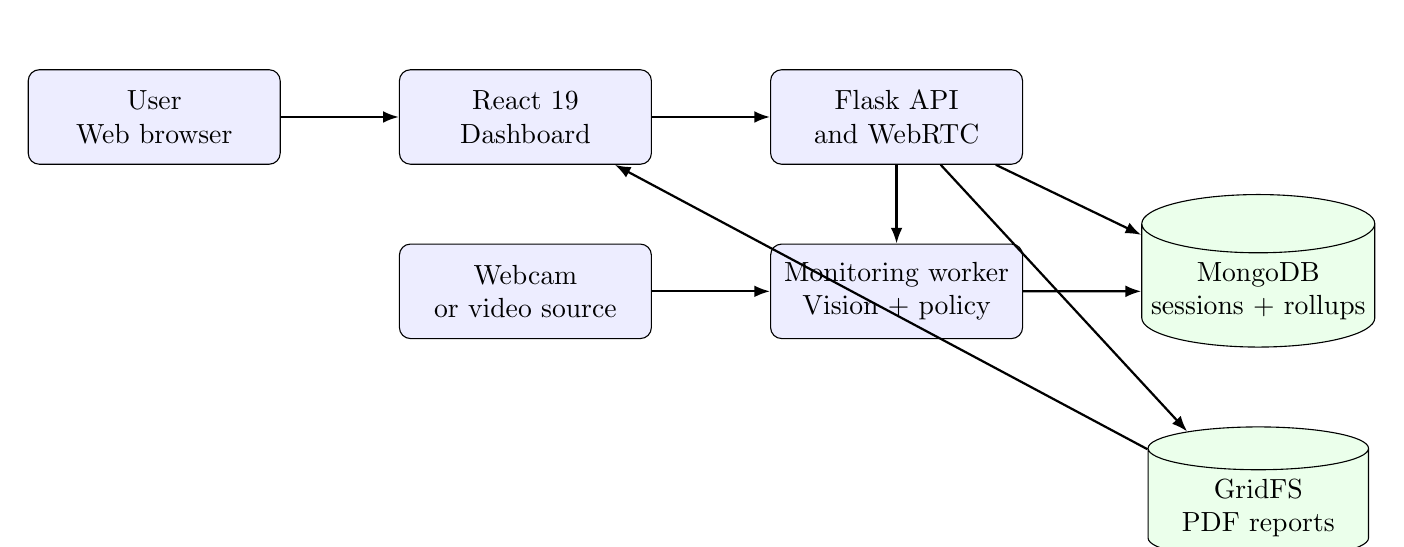
\begin{tikzpicture}[
node distance=10mm and 15mm,
box/.style={draw, rounded corners, fill=blue!7, align=center, minimum width=32mm, minimum height=12mm},
store/.style={draw, cylinder, shape border rotate=90, aspect=0.25, fill=green!8, align=center, minimum width=28mm, minimum height=13mm},
arrow/.style={-{Latex[length=2mm]}, thick}
]
\node[box] (user) {User\\Web browser};
\node[box, right=of user] (frontend) {React 19\\Dashboard};
\node[box, right=of frontend] (api) {Flask API\\and WebRTC};
\node[box, below=of api] (worker) {Monitoring worker\\Vision + policy};
\node[box, left=of worker] (camera) {Webcam\\or video source};
\node[store, right=of worker] (mongo) {MongoDB\\sessions + rollups};
\node[store, below=of mongo] (gridfs) {GridFS\\PDF reports};
\draw[arrow] (user) -- (frontend);
\draw[arrow] (frontend) -- (api);
\draw[arrow] (api) -- (worker);
\draw[arrow] (camera) -- (worker);
\draw[arrow] (worker) -- (mongo);
\draw[arrow] (api) -- (mongo);
\draw[arrow] (api) -- (gridfs);
\draw[arrow] (gridfs) -- (frontend);
\end{tikzpicture}
\caption{High-level system context}
\end{figure}

\section{Subsystems}
\begin{enumerate}
    \item \textbf{Capture and vision:} obtains frames and derives normalized
    measurements from face, iris, and pose landmarks.
    \item \textbf{Safety engine:} applies configured thresholds and temporal
    persistence to avoid flickering alerts.
    \item \textbf{Presentation:} annotates frames, updates live state, and
    sends notifications.
    \item \textbf{Telemetry:} writes local frame records and asynchronous
    one-second MongoDB rollups.
    \item \textbf{Reporting:} computes summary statistics, requests
    structured AI insights, renders charts, and creates a PDF.
    \item \textbf{Persistence and API:} manages users, sessions, telemetry,
    GridFS files, analytics, and authorization.
\end{enumerate}

\chapter{Low-Level Design}
\section{Monitoring Pipeline}
For each captured frame, the worker performs the following sequence:
\begin{enumerate}
    \item capture and mirror the image for natural selfie interaction;
    \item run the vision pipeline and attach a timestamp;
    \item evaluate the safety engine against the current temporal state;
    \item update the in-memory session reporter;
    \item append a detailed local JSONL record;
    \item add the record to the current one-second MongoDB bucket;
    \item annotate and publish the frame and live statistics; and
    \item trigger notifications when persistence conditions are met.
\end{enumerate}

\section{Vision Measurements}
\begin{table}[H]
\centering
\caption{Derived measurements and their use}
\begin{tabular}{p{0.28\textwidth}p{0.55\textwidth}}
\toprule
\textbf{Measurement} & \textbf{Use}\\
\midrule
Screen distance & Inverse calibrated model based on apparent face width.\\
Head pitch/yaw/roll & Detect neck and head orientation deviations.\\
Shoulder tilt & Detect asymmetry relative to calibrated neutral posture.\\
Slouch ratio & Estimate forward or collapsed upper-body posture.\\
Eye openness & Detect squinting and reduced eye comfort.\\
Blink rate & Estimate digital-wellness and visual-break behavior.\\
Gaze fixation & Detect unusually long motionless screen fixation.\\
Brightness strain & Classify dark-room, glare, and backlight conditions.\\
\bottomrule
\end{tabular}
\end{table}

\section{Temporal Policy}
Raw measurements are not immediately treated as a final user-facing status.
The safety engine keeps temporal state and requires a condition to persist
before escalating it. The conceptual state transition is:
\[
\mathrm{SAFE}\xrightarrow[\text{persistent warning}]{2s}
\mathrm{WARNING}\xrightarrow[\text{persistent hazard}]{5s}
\mathrm{NON\text{-}SAFE}.
\]
Recovery is intentionally faster than escalation so a transient good frame can
restore the user experience without excessive delay.

\section{Telemetry Rollup Algorithm}
The local JSONL record contains the detailed frame fields needed by the PDF
charts. The database record is formed by grouping frames by
\(\lfloor timestamp \rfloor\). For each second, the logger stores:
\begin{itemize}
    \item \code{sample\_count};
    \item arithmetic means for finite numeric fields;
    \item counts for each final status;
    \item counts for each policy reason; and
    \item the dominant final status.
\end{itemize}
When the timestamp changes, the completed bucket is submitted to a single
worker thread. The close operation waits for pending futures and reports
failures explicitly. If a session processes \(F\) frames at \(r\) frames per
second for \(T\) seconds, the MongoDB write count changes from approximately
\(F=rT\) documents to approximately \(T\) documents.

\begin{lstlisting}[language=Python,caption={Conceptual rollup persistence}]
bucket_start = int(record["timestamp"])
if bucket_start != current_bucket["bucket_start"]:
    queue_async(current_bucket)
    current_bucket = new_bucket(bucket_start)
update_averages_and_counts(current_bucket, record)
\end{lstlisting}

\chapter{Data and Persistence Design}
\section{MongoDB Collections}
\begin{table}[H]
\centering
\caption{Persistence model}
\begin{tabular}{p{0.23\textwidth}p{0.62\textwidth}}
\toprule
\textbf{Collection} & \textbf{Responsibilities}\\
\midrule
users & Credentials and user identity data.\\
sessions & Ownership, timestamps, duration, final statistics, PDF reference.\\
telemetry & One-second aggregate documents keyed by session and timestamp.\\
fs.files / fs.chunks & Generated PDF reports through GridFS.\\
\bottomrule
\end{tabular}
\end{table}

\section{Telemetry Document}
\begin{lstlisting}[language={},caption={Representative compact telemetry document}]
{
  "session_id": "665...",
  "user_id": "user-123",
  "bucket_start": 1730000000,
  "timestamp": 1730000000,
  "frame_index": 120,
  "sample_count": 30,
  "estimated_distance_cm": 61.2,
  "head_pitch_deg": -4.8,
  "shoulder_tilt_deg": 3.1,
  "blink_rate_per_min": 14.0,
  "status_counts": {"SAFE": 25, "WARNING": 5},
  "reason_counts": {"head_pitch_warning": 5},
  "final_status": "SAFE"
}
\end{lstlisting}

\section{Indexes and Query Patterns}
The telemetry collection is indexed by \((session\_id, timestamp)\) for
timeline reads and by \((user\_id)\) for user-scoped analytics. Session
documents are indexed by \((user\_id, started\_at)\). Timeline endpoints
downsample bucket records only when the requested point limit is exceeded;
they do not need to fetch thousands of frame-level documents.

\section{Retention and Cost Model}
The recommended operational policy is to retain compact rollups for the
product's history window and delete sessions through the authenticated delete
endpoint when the user requests removal. Local JSONL files are operational
artifacts and should be rotated or deleted after report generation according
to the deployment's retention policy. PDF files are separate GridFS objects
and are deleted with their owning session.

\chapter{API and Frontend Design}
\section{REST Resources}
\begin{longtable}{p{0.31\textwidth}p{0.47\textwidth}}
\toprule
\textbf{Endpoint} & \textbf{Purpose}\\
\midrule
\code{POST /api/auth/signup} & Create an account.\\
\code{POST /api/auth/login} & Authenticate and issue a token.\\
\code{POST /api/start} & Create a session and start monitoring.\\
\code{POST /api/stop} & Stop monitoring and begin report generation.\\
\code{GET /api/status} & Read current live worker state.\\
\code{GET /api/sessions} & List authenticated user's sessions.\\
\code{GET /api/sessions/<id>} & Read one owned session.\\
\code{GET /api/sessions/<id>/telemetry} & Read bucketed timeline data.\\
\code{GET /api/sessions/<id>/pdf} & Stream the stored GridFS PDF.\\
\code{GET /api/sessions/analytics/summary} & Read period analytics.\\
\code{DELETE /api/sessions/<id>} & Delete session, telemetry, and PDF.\\
\bottomrule
\end{longtable}

\section{Request and Report Sequence}
\begin{figure}[H]
\centering
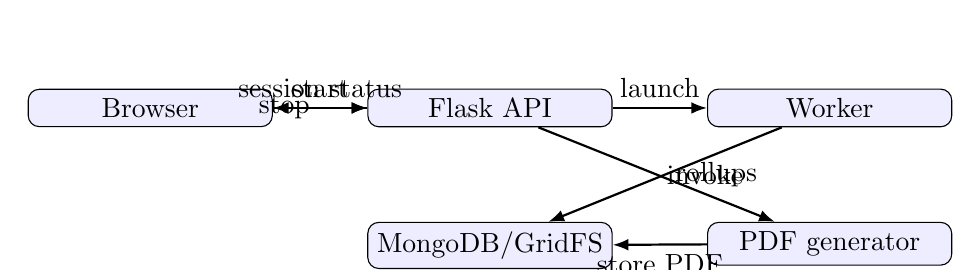
\begin{tikzpicture}[
node distance=12mm,
actor/.style={draw, rounded corners, fill=blue!7, minimum width=31mm, align=center},
arrow/.style={-{Latex[length=2mm]}, thick}
]
\node[actor] (browser) {Browser};
\node[actor, right=of browser] (api) {Flask API};
\node[actor, right=of api] (worker) {Worker};
\node[actor, below=of worker] (pdf) {PDF generator};
\node[actor, below=of api] (db) {MongoDB/GridFS};
\draw[arrow] (browser) -- node[above]{start} (api);
\draw[arrow] (api) -- node[above]{launch} (worker);
\draw[arrow] (worker) -- node[right]{rollups} (db);
\draw[arrow] (browser) -- node[left]{stop} (api);
\draw[arrow] (api) -- node[right]{invoke} (pdf);
\draw[arrow] (pdf) -- node[below]{store PDF} (db);
\draw[arrow] (api) -- node[above]{session status} (browser);
\end{tikzpicture}
\caption{Session and report generation sequence}
\end{figure}

\section{Frontend Responsibilities}
The React application is organized around authenticated pages for live
monitoring, dashboard analytics, session history, and report access. Live
metrics are intentionally separate from the video transport. This allows the
video stream to remain smooth even if a REST poll is delayed. The dashboard
uses the bucketed telemetry returned by the API for charts, so chart rendering
does not recreate frame-level storage pressure.

\chapter{Security, Privacy, and Safety}
\section{Authentication and Authorization}
Authentication is implemented through token-based protected routes. Each
session query includes the authenticated user identifier, and ownership is
checked before returning session details, telemetry, or PDF content. Delete
operations remove the session's associated GridFS object and telemetry records.

\section{Secret Management}
API keys, JWT secrets, and MongoDB connection strings must be loaded from
environment variables. The \code{.env} file is excluded by \code{.gitignore}
and must never be committed. Any credential that has been exposed in a chat,
terminal, log, or repository snapshot must be rotated immediately.

\section{Privacy Principles}
The system should collect only data required for posture feedback and the
user-requested report. Camera frames are processed in memory and are not
persisted by the described telemetry logger. Stored records contain derived
measurements, not raw camera imagery. Users should be informed about session
recording, retention, and deletion behavior.

\section{Wellness Safety}
AI-generated recommendations are grounded in summary telemetry and must be
presented as general ergonomic coaching. The report must not claim diagnosis,
medical certainty, or clinical treatment. When measurements are unavailable,
the system should identify missing data rather than manufacture a confident
result.

\chapter{Testing and Quality Assurance}
\section{Testing Strategy}
\begin{itemize}
    \item \textbf{Unit tests} validate distance, pose, temporal persistence,
    telemetry logging, and summary report generation.
    \item \textbf{Integration tests} exercise the pipeline from a representative
    frame through safety evaluation and reporting.
    \item \textbf{API tests} verify authentication, ownership, session
    lifecycle, analytics, and PDF access.
    \item \textbf{Regression tests} verify that two frames in one second become
    one MongoDB bucket and that weighted analytics remain correct.
    \item \textbf{Manual acceptance tests} verify browser video, alert timing,
    report download, and deletion behavior.
\end{itemize}

\section{Representative Test Matrix}
\begin{longtable}{p{0.22\textwidth}p{0.54\textwidth}p{0.13\textwidth}}
\toprule
\textbf{Area} & \textbf{Scenario} & \textbf{Expected}\\
\midrule
Vision & Face not detected & Safe fallback with explicit unknown state.\\
Policy & Hazard persists beyond threshold & Escalate to NON-SAFE.\\
Telemetry & 30 frames share one second & One aggregate document, count 30.\\
Analytics & Rollups have different sample counts & Weighted average.\\
Security & User requests another user's session & HTTP 404/denial.\\
Reporting & Empty telemetry file & Explicit failure, no fake report.\\
Lifecycle & Stop worker with pending writes & Close waits for writes.\\
\bottomrule
\end{longtable}

\section{Observed Session Example}
The supplied session summary contains 193 processed frames over 90.4 seconds,
with a posture score of 76.7 percent. It reports 60.1 percent SAFE, 33.2
percent WARNING, and 6.7 percent NON-SAFE frames. The most frequent recorded
issues are head pitch warning, shoulder tilt warning, slouch, and low blink
rate. These results demonstrate why both frequency and duration are useful:
the report can show trends while the policy engine avoids reacting to a
single noisy frame.

\chapter{Deployment and Operations}
\section{Runtime Components}
The backend requires Python dependencies for computer vision, Flask, WebRTC,
MongoDB, PDF rendering, and AI insight generation. The frontend requires a
Node.js environment and its package manifest. Production deployment should
place the API behind TLS and configure CORS to the known frontend origin.

\section{Startup Flow}
\begin{enumerate}
    \item Load environment configuration and validate required secrets.
    \item Initialize Flask routes and MongoDB indexes.
    \item Authenticate the user through the web dashboard.
    \item Create a session document when monitoring starts.
    \item Run the worker until an explicit stop or capture failure.
    \item Close local telemetry, flush rollups, and generate the report.
    \item Store the PDF in GridFS and update the session document.
\end{enumerate}

\section{Failure Handling}
Camera failure stops the worker and marks the session as stopped where
possible. MongoDB bucket failures are reported explicitly and do not become
success-shaped fallbacks. PDF generation failures leave the session available
with its final statistics while indicating that no PDF is available. This
separation prevents a reporting outage from corrupting the core monitoring
loop.

\section{Monitoring}
Operational metrics should include worker liveness, frame processing rate,
average inference duration, rollup queue depth, MongoDB write failures,
report-generation duration, and GridFS failures. Logs should avoid secrets and
raw personal data. A periodic cleanup job should enforce the chosen telemetry
and PDF retention window.

\chapter{Limitations and Future Enhancements}
\section{Current Limitations}
\begin{itemize}
    \item Webcam-based landmarks are sensitive to lighting, occlusion, camera
    angle, and partial visibility.
    \item A one-second rollup is appropriate for session analytics but cannot
    reproduce every frame-level event from MongoDB.
    \item AI insights depend on the availability, cost, and quota of the
    configured provider.
    \item The current report generator retains detailed local logs until the
    report is complete, so local disk cleanup remains an operational concern.
\end{itemize}

\section{Future Enhancements}
\begin{enumerate}
    \item Add configurable rollup intervals and retention policies.
    \item Compress or archive local JSONL files after PDF generation.
    \item Add a privacy-preserving on-device model mode with no cloud AI.
    \item Add calibration quality scoring and camera-placement guidance.
    \item Add alert acknowledgement and user-specific ergonomic goals.
    \item Add automated API contract and browser end-to-end testing.
    \item Add a time-series database only if scale justifies its operational
    cost; MongoDB rollups are sufficient for the current workload.
\end{enumerate}

\chapter{Conclusion}
The \systemname{} provides an end-to-end architecture for continuous
ergonomic feedback: computer vision generates measurements, temporal policy
turns measurements into stable guidance, the web dashboard exposes the
experience, and the reporting layer turns a session into actionable feedback.
The most important storage decision is the separation between detailed local
report input and compact database history. Persisting one aggregate per second
preserves averages, statuses, reason frequencies, and chart-level trends while
reducing database document growth by roughly the camera frame rate.

The design is therefore suitable as a maintainable academic project and as a
foundation for further hardening. Future work should prioritize privacy,
retention automation, calibration quality, comprehensive API tests, and
transparent user-facing explanations of the wellness recommendations.

\appendix
\chapter{Project Structure}
\begin{lstlisting}[language={}]
Major_Project/
|-- backend/
|   |-- api/
|   |-- app/
|   |-- reports/
|   |-- telemetry/
|   `-- generate_ai_pdf_report.py
|-- frontend/
|-- logs/
|-- tests/
|-- md_files/
|   |-- README.md
|   |-- explained.md
|   |-- ppt.md
|   |-- que_and.md
|   |-- frontend-README.md
|   `-- Project_Report.tex
`-- requirements.txt
\end{lstlisting}

\chapter{Glossary}
\begin{description}[style=nextline]
\item[EMA] Exponential moving average used to smooth measurements.
\item[GridFS] MongoDB storage mechanism for files larger than a document.
\item[HLD] High-Level Design describing system components and relationships.
\item[LLD] Low-Level Design describing algorithms, data, and module behavior.
\item[Rollup] Aggregate record representing a time bucket of raw observations.
\item[Telemetry] Measurements and decisions emitted by the monitoring system.
\item[WebRTC] Real-time browser media transport used for low-latency video.
\end{description}

\end{document}
